\titlecolor{Procédures de gestion de projet}
Une revue sera effectuée pendant chaque séance de travail planifiée à l'emploi du temps. Compte tenu de la courte durée de ces séances (2h), et en fonction de l'avancement du projet et de la date de la dernière revue, le chef de projet choisira de la faire au début ou à la fin de la séance. Cette revue permettra de faire un point oral sur l'avancement des tâches, de discuter d'éventuelles questions sur le projet, et de démarrer les nouvelles tâches. Elle servira également à préciser oralement ce qui devra être réalisé d'ici la prochaine séance de travail. Au besoin des réunions exceptionnelles pourront être décidées par le chef de projet entre deux séances de travail, avec toute ou partie de l'équipe. Les membres de l'équipe sont libres d'organiser leur temps de travail à leur souhait, les délais de fin des tâches ayant été fixés à l'avance, ils devront être respectés aux maximum.\\
Dès qu'un membre de l'équipe considère avoir terminé une de ces tâches, il doit prévenir le chef de projet qui validera alors le résultat de ce travail. Si un problème est trouvé, il sera corrigé par l'intervenant ayant réalisé le travail compte tenu du faible nombre de ressources dans le projet. Dès qu'un livrable est considéré comme complet par son rédacteur, qu'il soit le chef de projet ou un autre membre de l'équipe, il devra être relu par un autre membre de l'équipe pour détecter les erreurs de fond, les incohérences, mais également pour corriger les erreurs de forme, les fautes d'orthographe et les soucis de mise en page. Une fois le livrable relu, il sera validé par le chef de projet et pourra alors être présenter lors de la revue avec l'enseignant. Une fois tous les livrables validés par le chef de projet, ils pourront être livrés au client, sous forme numérique en un seul envoi groupé.\\

\titlecolor{Analyse des risques}
Afin d'essayer de prévoir les incidents qui pourraient empêcher le bon déroulement du projet et surtout de les éviter au maximum, nous listerons ci-dessous les risques identifiés.

\newpage
%\begin{figure}[!h]
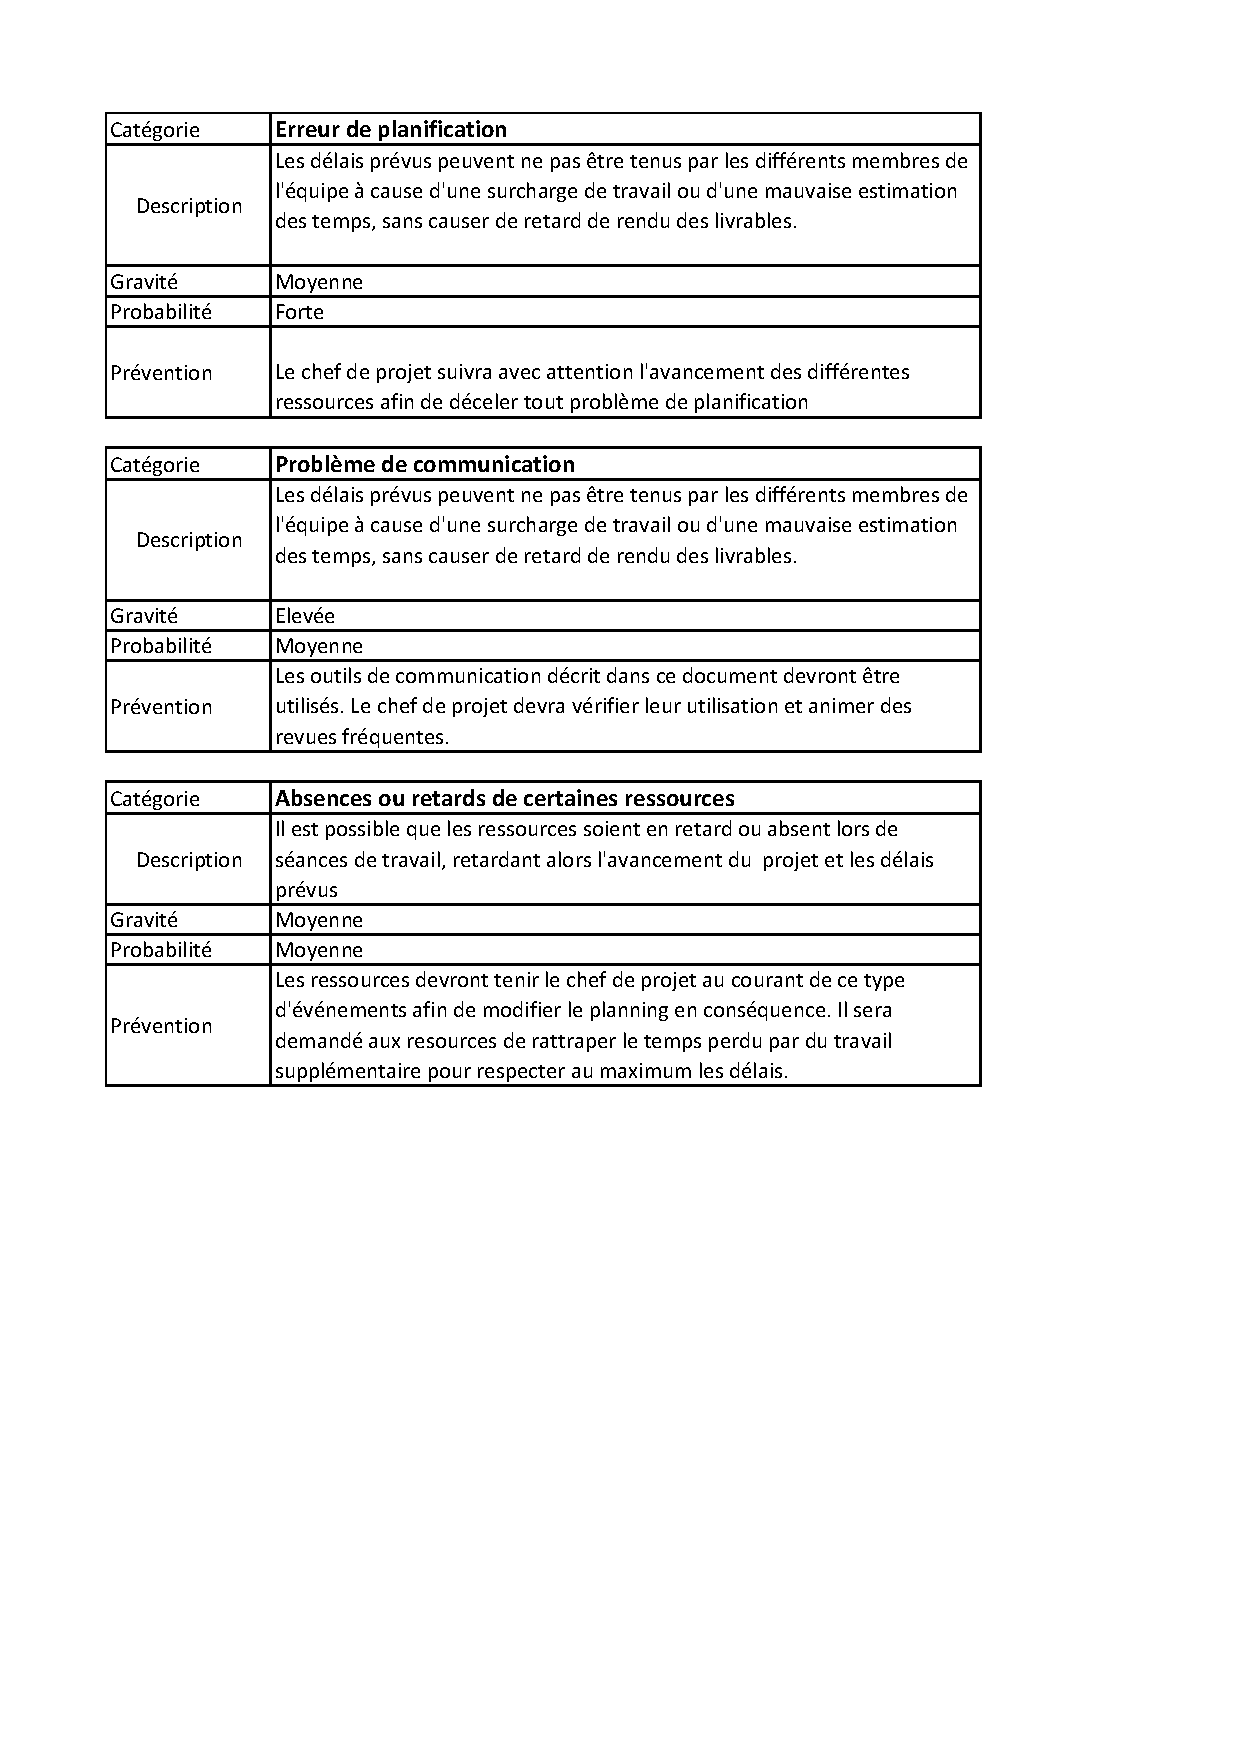
\includepdf [scale= 0.8] {Risques.pdf}
%\end{figure}